\chapter{المطيافية الدورانية والاهتزازية}\label{ch:b3:rovibrational-spectroscopy}

على هضبة عالية جافة، تتجه عشرات الهوائيات الراديوية نحو سحابة مظلمة
بين النجوم. ومن بين الترددات التي تلتقطها تردد عند
\qty{115.271}{GHz}: جزيئات أحادي أكسيد الكربون، عند بضعة كلفنات، تنتقل
من مستواها الدوراني الأول إلى الأدنى. ومن هذا العدد الوحيد يستخرج
الكيميائي طول الرابطة C--O بدقة جزء من البيكومتر؛ ومن
شدات الخطوط التالية، درجة حرارة السحابة. موضوع هذا الفصل
دورانات الجزيئات واهتزازاتها: مستوياتها، المأخوذة من الدوّار والهزاز في
\cref{ch:b3:quantum-model-systems}؛ وقواعد الانتقاء، المأخوذة من
\cref{ch:b3:group-theory-applied}؛ وما تقيسه الأطياف --- أطوال
الروابط، وثوابت القوة، وطاقات التفكك.

\begin{recall}
أعطى \cref{ch:b3:quantum-model-systems} \omterm{def:b3:quantum-model-systems:rotor}{الدوّار الصلب}، $E_J = J(J+1)\hbar^2/2I$
\omterm{def:b3:quantum-model-systems:degenerate}{بدرجة انحلال} $2J + 1$، \omterm{def:b3:quantum-model-systems:oscillator}{والهزاز التوافقي}، $E_v = (v + \frac12)h\nu$،
لجزيء ثنائي الذرة \omterm{def:b3:quantum-model-systems:oscillator}{كتلته المختزلة} $\mu$. وذكر \cref{ch:b3:group-theory-applied}
قواعد الانتقاء في تحت الأحمر ورامان. وقاس مجلد السنة الأولى أطياف تحت الأحمر
بالأعداد الموجية وعرّف قابلية استقطاب الجزيء.
\end{recall}

\begin{omfigure}
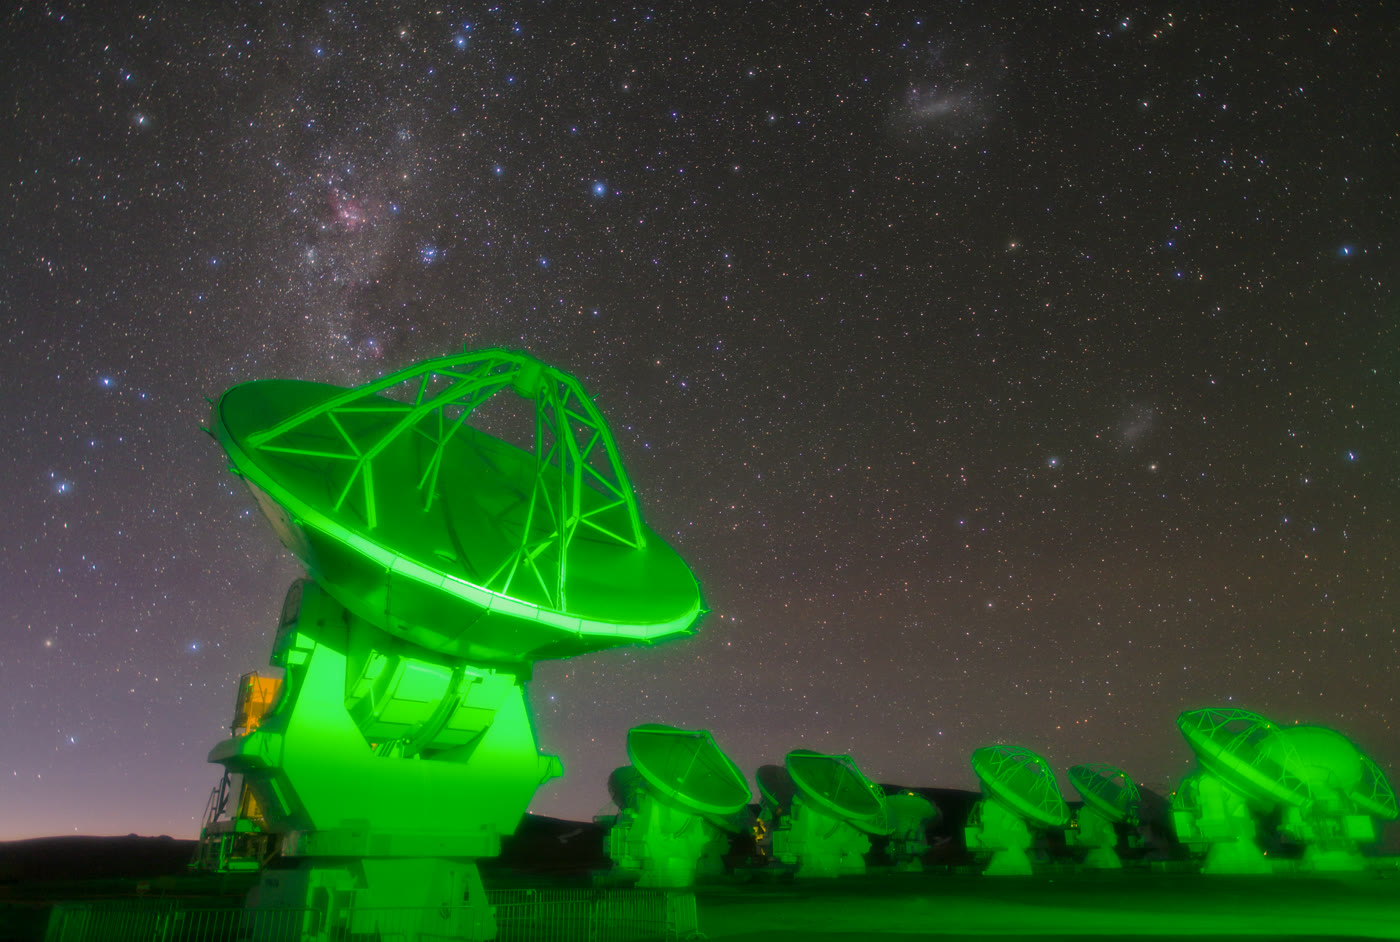
\includegraphics[width=0.7\linewidth]{images/book4/alma-antennas.jpg}

{\small هوائيات مقياس تداخل راديوي على هضبة عالية: تسجّل،
من بين خطوط أخرى كثيرة، الخطوط الدورانية لأحادي أكسيد الكربون الآتية من السحب
بين النجمية. الصورة: ESO/ب.~تفرشي (\url{twanight.org})، CC BY 4.0.}
\end{omfigure}

\section{الأطياف الدورانية}

\begin{definition}[ثابت الدوران، النظير الجزيئي]\label{def:b3:rovibrational-spectroscopy:rotational-constant}
\emph{ثابت الدوران}\index{ثابت الدوران} لجزيء خطي
هو $B = h/(8\pi^2cI)$، بوحدة \unit{cm^{-1}} (أو $B = h/8\pi^2I$ بالهرتز)، فتكون
مستوياته الدورانية $F(J) = BJ(J+1)$ بالأعداد الموجية. والجزيئات التي لا تختلف
إلا في نظائر ذراتها \emph{نظائر جزيئية}\index{نظير جزيئي}
(\ce{^{12}C^{16}O}، \ce{^{13}C^{16}O})؛ وفي \omterm{def:b3:computational-chemistry:born-oppenheimer}{تقريب بورن--أوبنهايمر}
تشترك في أطوال الروابط وثوابت القوة نفسها.
\end{definition}

\begin{definition}[قاعدتا الانتقاء العامة والنوعية]\label{def:b3:rovibrational-spectroscopy:selection}
\emph{قاعدة الانتقاء العامة}\index{قاعدة الانتقاء العامة} تحدد الخاصية
التي يجب أن يملكها الجزيء كي يُظهر نوعًا من الأطياف أصلًا؛ 
و\emph{قاعدة الانتقاء النوعية}\index{قاعدة الانتقاء النوعية} تحدد
تغيرات العدد الكمي المسموح بها.
\end{definition}

\begin{proposition}[الأطياف الدورانية الصرفة]\label{prop:b3:rovibrational-spectroscopy:rotational-lines}
لا يكون للجزيء طيف دوراني صرف (في الأمواج الميكروية) إلا إذا كان له
عزم ثنائي قطب دائم؛ والقاعدة النوعية للجزيء الخطي هي $\Delta J
= \pm1$. وتقع خطوط الامتصاص عند
\[
\tilde\nu = F(J+1) - F(J) = 2B(J + 1), \qquad J = 0, 1, 2, \dots,
\]
وهي متساوية التباعد بمقدار $2B$.
\end{proposition}

\begin{proof}
يتم التآثر مع الضوء عبر عزم ثنائي القطب: فالجزيء الذي لا عزم ثنائي قطب
دائمًا له لا يملك ثنائي قطب متذبذبًا حين يدور. والقاعدة $\Delta J
= \pm1$ تأتي من انعدام $\int Y_{J'M'}^*\cos\theta\,Y_{JM}$ ما لم يكن $J' = J
\pm 1$ (فمركبة ثنائي القطب على امتداد $z$ تتحول كما تتحول $Y_{1,0}$)، ونقبلها دون برهان.
عندئذ $B(J+1)(J+2) - BJ(J+1) = 2B(J+1)$.
\end{proof}

\begin{method}[طول الرابطة من خط دوراني]\label{met:b3:rovibrational-spectroscopy:bond-length}
\begin{enumerate}
  \item من الخط $J + 1 \leftarrow J$ ذي التردد $\nu$، استنتج $B =
        \nu/2(J+1)$ (بالهرتز).
  \item احسب عزم العطالة $I = h/8\pi^2B$.
  \item ومع \omterm{def:b3:quantum-model-systems:oscillator}{الكتلة المختزلة} المحسوبة من كتل النظائر، $r = \sqrt{I/\mu}$.
\end{enumerate}
\end{method}

\begin{example}[أحادي أكسيد الكربون]\label{ex:b3:rovibrational-spectroscopy:co}
% ledger: rotl:CO.1-0, imass:O16
يقع الخط $J = 1 \leftarrow 0$ للجزيء \ce{^{12}C^{16}O} عند \qty{115271.20}{MHz}:
$B = \qty{57635.6}{MHz} = \qty{1.92252}{cm^{-1}}$، $I = \qty{1.4560e-46}{kg.m^2}$.
ومع $\mu = 12 \times 15.99491/27.99491 = \qty{6.85621}{u}$، يكون $r_0 = \qty{113.09}{pm}$.
وهذا الطول $r_0$ متوسط للرابطة على اهتزازها عند النقطة الصفرية، وهو أطول قليلًا
من طول التوازن $r_e$ (\cref{sec:b3:rovibrational-spectroscopy:real-bonds}).
\end{example}

\begin{definition}[ثابت التشوه الطارد المركزي]\label{def:b3:rovibrational-spectroscopy:centrifugal}
تتمدد الرابطة الدوّارة؛ فتصير المستويات $F(J) = BJ(J+1) - DJ^2(J+1)^2$،
حيث $D$ هو \emph{ثابت التشوه الطارد المركزي}\index{ثابت التشوه الطارد المركزي}،
وتتقارب الخطوط $2B(J+1) - 4D(J+1)^3$ ببطء عند
قيم $J$ الكبيرة.
\end{definition}

\begin{proposition}[الخط الأشد]\label{prop:b3:rovibrational-spectroscopy:jmax}
إذا تبعت شدات الخطوط إشغال المستوى الأدنى، $(2J+1)
\eu^{-hcBJ(J+1)/kT}$، كان المستوى الأكثر إشغالًا قرب
\[
J_{\max} \approx \sqrt{\frac{kT}{2hcB}} - \frac12.
\]
\end{proposition}

\begin{proof}
لنعامل $J$ متغيرًا متصلًا ولنشتق: $\frac{\dd}{\dd J}[(2J+1)\eu^{-aJ(J+1)}]
= [2 - a(2J+1)^2]\eu^{-aJ(J+1)}$ حيث $a = hcB/kT$؛ وهي تنعدم عند $(2J + 1)^2 =
2/a$.
\end{proof}

\begin{omfigure}
\begin{tikzpicture}
\begin{axis}[width=0.9\linewidth, height=4.8cm, xmin=0, xmax=70, ymin=0,
  ymax=1.12, ytick=\empty, axis x line=bottom, axis y line=left, ycomb,
  xlabel={\foreignlanguage{arabic}{العدد الموجي \babelsublr{(cm$^{-1}$)}}}, ylabel={\foreignlanguage{arabic}{الشدة النسبية}},
  tick label style={font=\small}, label style={font=\small}]
\addplot[omDef, very thick] table[x=nu, y=I] {figdata/out/bachelor-3-rotational-spectrum-co-30.dat};
\addplot[omThm, thick, xshift=1.2pt] table[x=nu, y=I] {figdata/out/bachelor-3-rotational-spectrum-co-300.dat};
\end{axis}
\end{tikzpicture}

{\small طيف الامتصاص الدوراني لأحادي أكسيد الكربون، خطوطه متباعدة
بمقدار $2B = \qty{3.845}{cm^{-1}}$، والشدات مأخوذة مساوية لإشغال
المستوى الأدنى، عند \qty{30}{K} (أزرق) و\qty{300}{K} (أحمر، مزاح قليلًا من أجل
الوضوح)، وكل درجة حرارة محجَّمة على خطها الأشد. عند \qty{30}{K} يكون الخط الأشد
$J = 3 \leftarrow 2$؛ وعند \qty{300}{K}، $J = 8 \leftarrow 7$.}
\end{omfigure}

\section{اهتزازات الروابط الحقيقية}\label{sec:b3:rovibrational-spectroscopy:real-bonds}

لا تخضع الرابطة الحقيقية لقانون هوك بعيدًا عن التوازن: فهي تلين حين
تُمطّ ثم تنكسر.

\begin{definition}[كمون مورس]\label{def:b3:rovibrational-spectroscopy:morse}
\emph{كمون مورس}\index{كمون مورس} هو $V(r) = D_e[1 -
\eu^{-\beta(r - r_e)}]^2$: توافقي قرب $r_e$ (\omterm{def:b3:quantum-model-systems:oscillator}{ثابت القوة} $2\beta^2D_e$)، 
ويؤول إلى حد التفكك $D_e$ عند $r$ الكبيرة.
\end{definition}

\begin{proposition}[مستويات هزاز مورس]\label{prop:b3:rovibrational-spectroscopy:morse-levels}
بالأعداد الموجية، المستويات الاهتزازية لهزاز مورس هي
\[
G(v) = \tilde\omega_e(v + \tfrac12) - \tilde\omega_ex_e(v + \tfrac12)^2, \qquad
\tilde\omega_ex_e = \frac{\tilde\omega_e^2}{4D_e},
\]
وهي سلّم تتقارب درجاته وينتهي عند $v_{\max} = \lfloor\tilde\omega_e/
2\tilde\omega_ex_e - \frac12\rfloor$.
\end{proposition}
\admitted

يُتناول حل معادلة مورس في مقررات أكثر تقدمًا؛ 
والمستويات مُتحقَّق منها عدديًا في معطيات أشكال هذا الفصل.

\begin{definition}[ثابت اللاتوافقية، الانتقال الأساسي، النغمة التوافقية، الحزمة الساخنة]\label{def:b3:rovibrational-spectroscopy:anharmonic}
$\tilde\omega_ex_e$ هو \emph{ثابت اللاتوافقية}\index{ثابت اللاتوافقية}.
و\emph{الانتقال الأساسي}\index{انتقال أساسي}
هو $v = 1 \leftarrow 0$؛ و\emph{النغمة التوافقية}\index{نغمة توافقية} هي $v = n \leftarrow 0$
مع $n \ge 2$، وهي ضعيفة لأن القاعدة العامة $\Delta v = \pm1$ \omterm{def:b3:quantum-model-systems:oscillator}{للهزاز
التوافقي} لا تُخرق إلا قليلًا؛ و\emph{الحزمة الساخنة}\index{حزمة ساخنة} تنطلق
من مستوى مثار، $v = 2 \leftarrow 1$، وتشتد مع درجة الحرارة.
\end{definition}

\begin{definition}[طاقة التفكك الطيفية]\label{def:b3:rovibrational-spectroscopy:dissociation}
\emph{طاقة التفكك الطيفية}\index{طاقة التفكك الطيفية}
لجزيء هي عمق كمونه، $D_e$، مقيسًا من
القاع، أو $D_0 = D_e - G(0)$، مقيسًا من المستوى الأدنى --- لكل
جزيء عند \qty{0}{K}، خلافًا لأنتالبي تفكك الرابطة في مجلد السنة
الثانية، وهو أنتالبي مولي عند \qty{298}{K}.
\end{definition}

\begin{corollary}[$D_e$ و$D_0$ لهزاز مورس]\label{cor:b3:rovibrational-spectroscopy:de}
$D_e = \tilde\omega_e^2/4\tilde\omega_ex_e$ و$D_0 = D_e - (\frac12\tilde\omega_e -
\frac14\tilde\omega_ex_e)$.
\end{corollary}

\begin{proof}
الأولى هي علاقة القضية؛ والثانية هي $G(0)$.
\end{proof}

\begin{proposition}[استكمال بيرج--سبونر]\label{prop:b3:rovibrational-spectroscopy:birge-sponer}
الفجوات $\Delta G(v + \frac12) = G(v+1) - G(v) = \tilde\omega_e - 2\tilde\omega_ex_e(v +
1)$ تتناقص خطيًا مع $v$؛ ومجموعها حتى تنعدم يعطي $D_0$، أي
المساحة تحت منحنى $\Delta G$ بدلالة $v$.
\end{proposition}

\begin{proof}
لنطرح عبارتي $G$. و$D_0$ هي الطاقة من $v = 0$ إلى
الحد، أي مجموع كل الفجوات.
\end{proof}

\begin{example}[كلوريد الهيدروجين]\label{ex:b3:rovibrational-spectroscopy:hcl}
% ledger: diat:HCl.we, diat:HCl.wexe, janaf:H.dfH0, janaf:Cl.dfH0, janaf:HCl.dfH0
من أجل \ce{H^{35}Cl}، $\tilde\omega_e = \qty{2990.95}{cm^{-1}}$ و$\tilde\omega_ex_e =
\qty{52.82}{cm^{-1}}$: يقع \omterm{def:b3:rovibrational-spectroscopy:anharmonic}{الانتقال الأساسي} عند $\tilde\omega_e - 2\tilde\omega_ex_e =
\qty{2885.3}{cm^{-1}}$ \omterm{def:b3:rovibrational-spectroscopy:anharmonic}{والنغمة التوافقية} الأولى عند $2\tilde\omega_e - 6\tilde\omega_ex_e =
\qty{5665.0}{cm^{-1}}$، أي أقل قليلًا من ضعف الأساسي. ويتنبأ نموذج مورس
بالقيمتين $D_e = \qty{42342}{cm^{-1}}$ و$D_0 = \qty{40860}{cm^{-1}}$؛ أما $D_0$ الحقيقية،
المحسوبة من أنتالبيات تكوين H وCl وHCl عند \qty{0}{K}، فهي
\qty{35760}{cm^{-1}} (\qty{4.43}{eV}). فالكمون الحقيقي يتسطح أسرع من
منحنى مورس المضبوط عند القاع: واستكمالات بيرج--سبونر انطلاقًا من
المستويات الدنيا تبالغ في تقدير طاقات التفكك.
\end{example}

\begin{omfigure}
\begin{tikzpicture}
\begin{axis}[name=morse, width=0.55\linewidth, height=6cm, xmin=0.8, xmax=4.0,
  ymin=0, ymax=48000, axis lines=left, xlabel={\babelsublr{$r$ / \AA}}, ylabel={\babelsublr{$V$ / cm$^{-1}$}},
  unbounded coords=jump, scaled y ticks=false, ytick={0,10000,20000,30000,40000},
  tick label style={font=\small}, label style={font=\small}]
\addplot[black, thick] table[x=r, y=V] {figdata/out/bachelor-3-morse-levels.dat};
\addplot[gray, dashed] table[x=r, y=harm] {figdata/out/bachelor-3-morse-levels.dat};
\addplot[omDef] table[x=r, y=E] {figdata/out/bachelor-3-morse-levels-levels.dat};
\draw[<->, omThm] (axis cs:3.7,0) -- (axis cs:3.7,42342) node[pos=0.5, left, font=\small] {$D_e$};
\draw[dashed, omThm] (axis cs:1.2,42342) -- (axis cs:4.0,42342);
\end{axis}
\begin{axis}[at={(morse.east)}, anchor=west, xshift=1.6cm, width=0.4\linewidth,
  height=5cm, xmin=0, xmax=28, ymin=0, ymax=3100, axis lines=left,
  xlabel={$v$}, ylabel={\babelsublr{$\Delta G(v + \frac12)$ / cm$^{-1}$}},
  tick label style={font=\small}, label style={font=\small}]
\addplot[omDef, only marks, mark size=1.2pt] table[x=v, y=dG] {figdata/out/bachelor-3-morse-levels-bs.dat};
\addplot[omDef!40, fill=omDef!12, draw=none] table[x=v, y=dG] {figdata/out/bachelor-3-morse-levels-bs.dat} \closedcycle;
\end{axis}
\end{tikzpicture}

{\small يسارًا: \omterm{def:b3:rovibrational-spectroscopy:morse}{كمون مورس} للجزيء \ce{HCl} مبنيًا من ثوابته
الطيفية (متصل)، والقطع المكافئ التوافقي ذو الانحناء نفسه (متقطع)،
ومستوى اهتزازي من كل ثلاثة، مرسومًا بين نقطتي ارتداده؛ 
والمستويات تتقارب نحو $D_e$. يمينًا: منحنى بيرج--سبونر للفجوات؛
والمساحة المظللة هي $D_0$.}
\end{omfigure}

\section{الحزم الدورانية الاهتزازية}

يرافق الانتقالَ الاهتزازي في غاز تغيراتٌ دورانية، $\Delta
J = \pm1$ لجزيء ثنائي الذرة في حالة ${}^1\Sigma$.

\begin{definition}[الفروع P وQ وR، أصل الحزمة]\label{def:b3:rovibrational-spectroscopy:branches}
في الحزمة الدورانية الاهتزازية، تشكّل الخطوط ذات $\Delta J = -1$ \emph{الفرع
P}\index{الفرع P}، والخطوط ذات $\Delta J = +1$ \emph{الفرع R}\index{الفرع R}،
والخطوط ذات $\Delta J = 0$، حين تكون مسموحة، \emph{الفرع Q}\index{الفرع Q}.
و\emph{أصل الحزمة}\index{أصل الحزمة} $\tilde\nu_0$ هو
فرق الطاقة الاهتزازية دون دوران.
\end{definition}

\begin{theorem}[فروق التركيب]\label{thm:b3:rovibrational-spectroscopy:combination-differences}
إذا كان \omterm{def:b3:rovibrational-spectroscopy:rotational-constant}{ثابتا الدوران} $B_0$ و$B_1$ في المستويين الاهتزازيين الأدنى والأعلى،
فإن $R(J) = \tilde\nu_0 + B_1(J+1)(J+2) - B_0J(J+1)$ و$P(J) = \tilde\nu_0 +
B_1(J-1)J - B_0J(J+1)$، و
\[
R(J - 1) - P(J + 1) = 4B_0(J + \tfrac12), \qquad R(J) - P(J) = 4B_1(J + \tfrac12).
\]
\end{theorem}

\begin{proof}
تنتج العلاقتان الأوليان عن $E = G(v) + B_vJ(J+1)$ في المستويين كليهما. و$R(J - 1)$ 
و$P(J + 1)$ ينتهيان إلى المستوى الأعلى نفسه $J$، انطلاقًا من المستويين الأدنيين $J - 1$ و$J + 1$:
وفرقهما $B_0[(J+1)(J+2) - (J-1)J] = B_0(4J + 2)$. وبالمثل ينطلق $R(J)$ 
و$P(J)$ من المستوى الأدنى نفسه وينتهيان إلى $J + 1$ و$J - 1$.
\end{proof}

\begin{method}[تحليل حزمة دورانية اهتزازية]\label{met:b3:rovibrational-spectroscopy:combination}
\begin{enumerate}
  \item حدّد الفجوة: في جزيء ثنائي الذرة في حالة ${}^1\Sigma$ لا يوجد فرع Q، 
        و$\tilde\nu_0$ يقع في الفجوة، بين $R(0)$ و$P(1)$.
  \item رقّم الخطوط نحو الخارج انطلاقًا من الفجوة: $R(0), R(1), \dots$ و$P(1),
        P(2), \dots$.
  \item استعمل فروق التركيب للحصول على $B_0$ و$B_1$
        كل على حدة، ثم $\alpha_e = B_0 - B_1$ و$B_e = B_0 + \frac12\alpha_e$.
\end{enumerate}
\end{method}

\begin{omfigure}
\begin{tikzpicture}
\begin{axis}[width=0.92\linewidth, height=5cm, xmin=2650, xmax=3080, ymin=0,
  ymax=1.15, ytick=\empty, axis x line=bottom, axis y line=left,
  xlabel={\foreignlanguage{arabic}{العدد الموجي \babelsublr{(cm$^{-1}$)}}}, ylabel={\foreignlanguage{arabic}{الامتصاصية النسبية}},
  tick label style={font=\small}, label style={font=\small}]
\addplot[omDef, thin] table[x=nu, y=A] {figdata/out/bachelor-3-rovib-band.dat};
\node[font=\small] at (axis cs:2780,1.06) {\foreignlanguage{arabic}{الفرع P}};
\node[font=\small] at (axis cs:2985,1.06) {\foreignlanguage{arabic}{الفرع R}};
\draw[->, gray] (axis cs:2885.3,0.45) -- (axis cs:2885.3,0.05);
\node[font=\small, gray, anchor=south] at (axis cs:2885.3,0.45) {$\tilde\nu_0$};
\end{axis}
\end{tikzpicture}

{\small الحزمة الأساسية لغاز \ce{HCl} عند \qty{300}{K}، محسوبة من
ثوابته الطيفية: الفرعان P وR على جانبي الفجوة عند
\omterm{def:b3:rovibrational-spectroscopy:branches}{أصل الحزمة}. وكل خط ثنائي، \ce{H^{35}Cl} والخط الأضعف، الأدنى
قليلًا، \ce{H^{37}Cl} (الوفرتان الطبيعيتان 76\,\% و24\,\%). تتقارب خطوط R،
وتتباعد خطوط P، لأن $B_1 < B_0$.}
\end{omfigure}

\begin{example}[ثوابت \ce{HCl} من حزمته]\label{ex:b3:rovibrational-spectroscopy:analysis}
% ledger: diat:HCl.Be, diat:HCl.ae
بأخذ $R(0) = \qty{2905.58}{cm^{-1}}$ و$P(2) = \qty{2842.94}{cm^{-1}}$، نجد
$6B_0 = \qty{62.64}{cm^{-1}}$، ومنه $B_0 = \qty{10.440}{cm^{-1}}$. وبأخذ $R(1) = 2925.23$ و$P(1) =
\qty{2864.43}{cm^{-1}}$، $B_1 = \qty{10.133}{cm^{-1}}$. ومنه $\alpha_e = \qty{0.307}{cm^{-1}}$
و$B_e = \qty{10.593}{cm^{-1}}$، وهي القيم التي بُنيت منها الحزمة:
فالطريقة تستعيدها بالضبط.
\end{example}

\section{مطيافية رامان}

\begin{definition}[انتثار رامان وانتثار رايلي]\label{def:b3:rovibrational-spectroscopy:raman}
حين يعبر ضوء تردده $\nu_0$ عيّنةً، يحافظ معظم الضوء المنتثر
على التردد $\nu_0$: وهذا \emph{انتثار رايلي}\index{انتثار رايلي}.
ويُزاح جزء صغير بالترددات الدورانية أو الاهتزازية
للجزيئات: وهذا \emph{انتثار رامان}\index{انتثار رامان}.
والخطوط ذات التردد الأدنى \emph{خطوط ستوكس}\index{خط ستوكس} (فقد
اكتسب الجزيء طاقة)، وذات التردد الأعلى \emph{خطوط ضد
ستوكس}\index{خط ضد ستوكس} (فقد خسر طاقة).
\end{definition}

\begin{proposition}[المنشأ الكلاسيكي لمفعول رامان]\label{prop:b3:rovibrational-spectroscopy:raman-classical}
إذا تغيرت قابلية استقطاب جزيء يهتز بالتردد $\nu_{\mathrm{vib}}$
وفق $\alpha = \alpha_0 + \alpha_1\cos(2\pi\nu_{\mathrm{vib}}t)$، فإن ثنائي القطب الذي يحرّضه
مجال $E_0\cos(2\pi\nu_0t)$ يتذبذب بالتردد $\nu_0$ وبالترددين $\nu_0 \pm \nu_{\mathrm{vib}}$.
ولا يكون الاهتزاز \omterm{def:b3:group-theory-applied:activity}{نشطًا في رامان} إلا إذا غيّر قابلية الاستقطاب.
\end{proposition}

\begin{proof}
$\mu = \alpha E = \alpha_0E_0\cos(2\pi\nu_0t) + \frac12\alpha_1E_0[\cos2\pi(\nu_0 +
\nu_{\mathrm{vib}})t + \cos2\pi(\nu_0 - \nu_{\mathrm{vib}})t]$، بالعلاقة $\cos a\cos b =
\frac12[\cos(a+b) + \cos(a-b)]$. وكل ثنائي قطب متذبذب يشع بتردده
الخاص؛ ودون $\alpha_1$ لا يبقى إلا حد رايلي.
\end{proof}

\begin{proposition}[خطوط رامان الدورانية]\label{prop:b3:rovibrational-spectroscopy:rotational-raman}
يُظهر الجزيء الخطي ذو قابلية الاستقطاب غير المتماثلة الاتجاه خطوط رامان دورانية
تحقق $\Delta J = \pm2$، مزاحة عن خط الإثارة بمقدار
\[
|\Delta\tilde\nu| = F(J+2) - F(J) = 4B(J + \tfrac32) = 6B, 10B, 14B, \dots
\]
--- الخط الأول عند $6B$، ثم تباعد قدره $4B$.
\end{proposition}

\begin{proof}
يعود قطع ناقص الاستقطاب لجزيء خطي دوّار إلى
الاتجاه نفسه مرتين في كل دورة، فيعدّل الانتثار بضعف
تردد الدوران: $\Delta J = \pm2$ (القاعدة الكمومية، نقبلها دون برهان). عندئذ
$B(J+2)(J+3) - BJ(J+1) = B(4J + 6)$.
\end{proof}

\begin{example}[النيتروجين، كما يراه رامان]\label{ex:b3:rovibrational-spectroscopy:n2}
% ledger: diat:N2.Be, diat:N2.ae
ليس للجزيء \ce{N2} ثنائي قطب ولا طيف في تحت الأحمر أو في الأمواج الميكروية، لكن
قابلية استقطابه غير متماثلة الاتجاه: فخطوط رامان الدورانية له تبدأ عند $6B_0 =
\qty{11.94}{cm^{-1}}$ من خط الإثارة ويفصل بينها \qty{7.96}{cm^{-1}}. وتتناوب
شداتها بنسبة 2:1 بين قيم $J$ الزوجية والفردية: فنواتا \ce{^{14}N}
متطابقتان، وإحصاء سبين النوى (\cref{ch:b3:statistical-thermo-applied})
يعطي المستويات ذات $J$ الزوجي ضعف وزن المستويات الفردية.
\end{example}

\begin{omfigure}
\begin{tikzpicture}
\begin{axis}[name=r, width=0.55\linewidth, height=4.6cm, xmin=-110, xmax=110,
  ymin=0, ymax=1.1, ytick=\empty, axis x line=bottom, axis y line=left, ycomb,
  xlabel={\foreignlanguage{arabic}{انزياح رامان \babelsublr{(cm$^{-1}$)}}}, tick label style={font=\small}, label style={font=\small},
  title={\small \foreignlanguage{arabic}{\ce{N2}، رامان الدوراني، \qty{300}{K}}}]
\addplot[omDef, thick] table[x=shift, y=I] {figdata/out/bachelor-3-rotational-spectrum-n2-raman.dat};
\draw[gray, thick] (axis cs:0,0) -- (axis cs:0,1.05);
\end{axis}
\begin{scope}[xshift=0.6\linewidth, font=\small]
  \draw[omstate] (0,0) -- (2.4,0) node[right] {$v = 0$};
  \draw[omstate] (0,1.0) -- (2.4,1.0) node[right] {$v = 1$};
  \draw[omvib, densely dashed] (0,3.2) -- (2.4,3.2) node[right] {\foreignlanguage{arabic}{افتراضي}};
  \draw[omabs] (0.3,0) -- (0.3,3.18);
  \draw[omfluo] (0.5,3.18) -- (0.5,0.02);
  \node[font=\scriptsize, omThm, anchor=east] at (0.22,1.6) {\foreignlanguage{arabic}{رايلي}};
  \draw[omabs] (1.3,0) -- (1.3,3.18);
  \draw[omphos] (1.5,3.18) -- (1.5,1.02) node[pos=0.4, right, font=\scriptsize] {\foreignlanguage{arabic}{ستوكس}};
\end{scope}
\end{tikzpicture}

{\small يسارًا: طيف رامان الدوراني للنيتروجين محسوبًا عند
\qty{300}{K}: \omterm{def:b3:rovibrational-spectroscopy:raman}{خطوط ستوكس} عند الانزياحات الموجبة (يمينًا)، \omterm{def:b3:rovibrational-spectroscopy:raman}{وخطوط ضد ستوكس} عند
الانزياحات السالبة (يسارًا، أضعف قليلًا)، مع تناوب الشدات بنسبة 2:1؛
والخط الرمادي عند الصفر يدل على خط رايلي الأشد بكثير. يمينًا: مخطط طاقة \omterm{def:b3:rovibrational-spectroscopy:raman}{لانتثار رايلي} وانتثار ستوكس
عبر مستوى افتراضي (ليس حالة حقيقية للجزيء).}
\end{omfigure}

\section{الجزيئات المتعددة الذرات}

\begin{definition}[أنواع الدوّارات]\label{def:b3:rovibrational-spectroscopy:rotor-types}
الجزيء الذي عزوم عطالته الرئيسية الثلاثة متساوية
\emph{خذروف كروي}\index{خذروف كروي} (\ce{CH4}، \ce{SF6})؛ وإذا تساوى اثنان منها فهو
\emph{خذروف متناظر}\index{خذروف متناظر} (\ce{NH3}، \ce{CHCl3}، \ce{C6H6})؛
وإذا اختلفت الثلاثة فهو \emph{خذروف لامتناظر}\index{خذروف لامتناظر}
(\ce{H2O}، ومعظم الجزيئات)؛ وللجزيئات الخطية عزم معدوم.
\end{definition}

ليس \omterm{def:b3:rovibrational-spectroscopy:rotor-types}{للخذروف الكروي} ثنائي قطب ولا طيف دوراني؛ وللخذروف المتناظر
مستويات $BJ(J+1) + (A - B)K^2$، حيث يعدّ $K$ كمية الحركة الزاوية حول محوره،
وخطوط تقع دائمًا عند $2B(J+1)$ لأن $\Delta K = 0$؛ أما \omterm{def:b3:rovibrational-spectroscopy:rotor-types}{الخذروف اللامتناظر}
فطيفه غير منتظم، يُضبط بالحاسوب. واهتزازات الجزيئات المتعددة الذرات
هي أنماطها العادية، المسمّاة والمنتقاة في
\cref{ch:b3:group-theory-applied}: فطيف تحت الأحمر يُظهر الأنماط
التي تتحول كما تتحول $x$ و$y$ و$z$، ولكل منها بنيته الدورانية.

\begin{inthelab}[خلية غاز في مطياف تحت الأحمر]
يُدخل غاز \ce{HCl} في خلية طولها \qty{10}{cm} ذات نوافذ شفافة في
تحت الأحمر، داخل مطياف بتحويل فورييه. وبميز \qty{1}{cm^{-1}}
يظهر الفرعان P وR خطوطًا مفردة؛ وبميز \qty{0.25}{cm^{-1}} ينشطر كل خط
إلى ثنائيته \ce{H^{35}Cl} و\ce{H^{37}Cl}، المتباعدة \qty{2}{cm^{-1}}. وكلوريد
الهيدروجين سام وأكّال: فتُملأ الخلية على خط تفريغ تحت ساحبة
الأبخرة.
\end{inthelab}

\begin{safety}{\ghs[0.8cm]{GHS04}\ghs[0.8cm]{GHS05}\ghs[0.8cm]{GHS06}}
غاز كلوريد الهيدروجين: غاز تحت ضغط، أكّال للجلد والعينين 
والمسالك التنفسية، سام إذا استُنشق. لا يُتداول إلا في جهاز مغلق أو تحت
ساحبة الأبخرة.
\end{safety}

\begin{history}[رامان، 1928]
في سنة 1928 رصد ش. ف. رامان وك. س. كريشنان، في ضوء الشمس المرشَّح عبر
مرشح بنفسجي والمنتثر في سوائل، ضوءًا خافتًا من لون مختلف
يستطيع مرشح أخضر متصالب أن يعزله. ونال رامان جائزة نوبل في الفيزياء لسنة 1930؛
وحوّلت مصادر الليزر مفعوله إلى تقنية تحليلية
روتينية بعد خمسين سنة.
\end{history}

\section{تمارين}

\begin{exercise}[$\star$]\label{exo:b3:rovibrational-spectroscopy:1}
% ledger: imass:O16
انطلاقًا من $B_0 = \qty{1.9225}{cm^{-1}}$ للجزيء \ce{^{12}C^{16}O}، احسب عزم العطالة
وطول الرابطة $r_0$.
\end{exercise}

\begin{exercise}[$\star$]\label{exo:b3:rovibrational-spectroscopy:2}
% ledger: diat:HCl.Be, diat:HCl.ae
بأخذ $B_0 = \qty{10.440}{cm^{-1}}$، أعطِ مواضع الخطوط الأربعة الأولى في
الطيف الدوراني للجزيء \ce{H^{35}Cl} وقيمة $J$ للخط الأشد عند
\qty{300}{K}.
\end{exercise}

\begin{exercise}[$\star$]\label{exo:b3:rovibrational-spectroscopy:3}
أيّ الجزيئات \ce{H2} و\ce{HCl} و\ce{N2} و\ce{CO2} و\ce{CH4} و\ce{SF6} و\ce{H2O} يُظهر طيف امتصاص
دورانيًا صرفًا؟ وأيها يُظهر طيف رامان دورانيًا؟
\end{exercise}

\begin{exercise}[$\star$]\label{exo:b3:rovibrational-spectroscopy:4}
% ledger: diat:HCl.we, diat:HCl.wexe
ما نسبة جزيئات \ce{HCl} الموجودة في $v = 1$ عند 300 و\qty{1000}{K}
(\omterm{def:b3:rovibrational-spectroscopy:anharmonic}{الانتقال الأساسي} \qty{2885.3}{cm^{-1}})؟ ومتى تصبح \omterm{def:b3:rovibrational-spectroscopy:anharmonic}{الحزمة الساخنة} مرئية؟
\end{exercise}

\begin{exercise}[$\star\star$]\label{exo:b3:rovibrational-spectroscopy:5}
يقع \omterm{def:b3:rovibrational-spectroscopy:anharmonic}{الانتقال الأساسي} \omterm{def:b3:rovibrational-spectroscopy:anharmonic}{والنغمة التوافقية} الأولى للجزيء \ce{H^{35}Cl} عند 2885.3 
و\qty{5665.0}{cm^{-1}}. استنتج $\tilde\omega_e$ و$\tilde\omega_ex_e$.
\end{exercise}

\begin{exercise}[$\star\star$]\label{exo:b3:rovibrational-spectroscopy:6}
بثوابت التمرين السابق، احسب $D_e$ و$D_0$ في
نموذج مورس، وقارن بالقيمة الحقيقية $D_0 = \qty{35760}{cm^{-1}}$. وحوّل قيمتي
$D_0$ كلتيهما إلى \unit{kJ/mol}.
\end{exercise}

\begin{exercise}[$\star\star$]\label{exo:b3:rovibrational-spectroscopy:7}
أربعة خطوط من الحزمة الأساسية للجزيء \ce{H^{35}Cl} هي $R(0) = 2905.58$، $R(1) = 2925.23$،
$P(1) = 2864.43$ و$P(2) = \qty{2842.94}{cm^{-1}}$. جد $B_0$ و$B_1$ و$\alpha_e$ 
\omterm{def:b3:rovibrational-spectroscopy:branches}{وأصل الحزمة}.
\end{exercise}

\begin{exercise}[$\star\star$]\label{exo:b3:rovibrational-spectroscopy:8}
% ledger: imass:H1, imass:H2, imass:Cl35
تنبأ بقيمة $B_0$ وبأصل الحزمة للجزيء \ce{D^{35}Cl} انطلاقًا من قيمتيهما للجزيء \ce{H^{35}Cl}، مستعملًا
الكتل المختزلة ($\tilde\omega_e \propto \mu^{-1/2}$، $\tilde\omega_ex_e \propto
\mu^{-1}$، $B \propto \mu^{-1}$).
\end{exercise}

\begin{exercise}[$\star\star$]\label{exo:b3:rovibrational-spectroscopy:9}
% ledger: diat:N2.Be, diat:N2.ae
من أجل \ce{N2}، $B_0 = \qty{1.9896}{cm^{-1}}$. أعطِ انزياحات خطوط رامان الدورانية
الثلاثة الأولى من نوع ستوكس، وفسّر تناوب
شداتها.
\end{exercise}

\begin{exercise}[$\star\star\star$]\label{exo:b3:rovibrational-spectroscopy:10}
% ledger: rotl:CO.1-0, rotl:CO.2-1, rotl:CO.3-2
الخطوط الدورانية الثلاثة الأولى للجزيء \ce{^{12}C^{16}O} تقع عند 115271.2018 
و230538.0000 و\qty{345795.9899}{MHz}. بيّن أن \omterm{def:b3:quantum-model-systems:rotor}{الدوّار الصلب} لا يوافقها،
وعيّن $B$ \omterm{def:b3:rovibrational-spectroscopy:centrifugal}{وثابت التشوه الطارد المركزي} $D$.
\end{exercise}

\begin{exercise}[$\star\star\star$]\label{exo:b3:rovibrational-spectroscopy:11}
بيّن أن مجموع بيرج--سبونر للفجوات $\Delta G(v + \frac12)$ لهزاز مورس
من $v = 0$ إلى آخر مستوى مقيَّد قريب من $D_e - G(0)$، 
واحسب المجموع من أجل \ce{HCl}.
\end{exercise}

\begin{exercise}[$\star\star\star$]\label{exo:b3:rovibrational-spectroscopy:12}
سبين نواة \ce{^{16}O} معدوم، فلا وجود لمستويات \ce{^{16}O^{12}C^{16}O} ذات
$J$ الفردي. ما تباعد خطوط رامان الدورانية فيه، وما
انزياح الخط الأول، بدلالة $B$؟ ولماذا ليس للجزيء \ce{CO2} طيف في
الأمواج الميكروية؟
\end{exercise}

\section{مسألة: الإصغاء إلى سحابة باردة}

\begin{problem}[{مسألة نهاية الأسبوع --- طول رابطة أحادي أكسيد الكربون من
خطه الدوراني الأول، ودرجة حرارة سحابة بين نجمية، والنظير
الجزيئي ذو الكربون-13، والحزمة تحت الحمراء}]
\label{pb:b3:rovibrational-spectroscopy:1}
% ledger: rotl:CO.1-0, rotl:CO.2-1, rotl:13CO.1-0, imass:O16, imass:C13, iso:C13, diat:CO.we, diat:CO.wexe, re:CO
المعطيات: خطا \ce{^{12}C^{16}O}، $J = 1 \leftarrow 0$ عند \qty{115.2712}{GHz} و$2
\leftarrow 1$ عند \qty{230.5380}{GHz}؛ وخط \ce{^{13}C^{16}O}، $1 \leftarrow 0$ عند
\qty{110.2014}{GHz}؛ والكتل \ce{^{12}C} 12 (بالضبط)، و\ce{^{13}C} 13.00335،
و\ce{^{16}O} \qty{15.99491}{u}؛ والوفرة الطبيعية للنظير \ce{^{13}C} 1.1\,\%؛ ومن أجل \ce{^{12}C^{16}O}،
$\tilde\omega_e = \qty{2169.81}{cm^{-1}}$، $\tilde\omega_ex_e = \qty{13.288}{cm^{-1}}$، 
وطول التوازن $r_e = \qty{112.83}{pm}$. $h = \qty{6.62607e-34}{J.s}$، $u =
\qty{1.66054e-27}{kg}$، $c = \qty{2.99792e10}{cm/s}$، $hc/k = \qty{1.43878}{cm.K}$.

\medskip\noindent\textbf{الجزء الأول --- الرابطة.}
\begin{enumerate}
  \item احسب $B_0$ بالهرتز وبوحدة \unit{cm^{-1}}.
  \item احسب \omterm{def:b3:quantum-model-systems:oscillator}{الكتلة المختزلة} للجزيء \ce{^{12}C^{16}O} بالكيلوغرام.
  \item احسب عزم العطالة.
  \item استنتج $r_0$.
  \item قارن بالطول $r_e$. لماذا يكون $r_0$ أطول؟
  \item تنبأ بموضع الخط $2 \leftarrow 1$ من أجل \omterm{def:b3:quantum-model-systems:rotor}{دوّار صلب}. وعلّق على
        القيمة المقيسة.
\end{enumerate}

\medskip\noindent\textbf{الجزء الثاني --- درجة حرارة السحابة.}
\begin{enumerate}[resume]
  \item أعطِ، بوحدة \unit{cm^{-1}} وبالكلفن ($E/k$)، طاقات المستويات $J =
        0$ و1 و2.
  \item اكتب نسبة الإشغالين $N_2/N_1$ عند درجة الحرارة $T$.
  \item تعطي الأرصاد $N_2/N_1 = 0.85$ (معطيات المسألة). جد $T$.
  \item أي مستوى هو الأكثر إشغالًا عند درجة الحرارة هذه؟
  \item لماذا لا يمكن رؤية مثل هذه السحابة في الحزمة الاهتزازية تحت الحمراء؟
  \item لماذا يكون الخط $1 \leftarrow 0$ أكثر الكواشف استعمالًا لتتبع الغاز البارد؟
\end{enumerate}

\medskip\noindent\textbf{الجزء الثالث --- \omterm{def:b3:rovibrational-spectroscopy:rotational-constant}{النظير الجزيئي}.}
\begin{enumerate}[resume]
  \item احسب \omterm{def:b3:quantum-model-systems:oscillator}{الكتلة المختزلة} للجزيء \ce{^{13}C^{16}O}.
  \item تنبأ بخطه $1 \leftarrow 0$ انطلاقًا من خط \ce{^{12}C^{16}O}.
  \item قارن بالقيمة المقيسة \qty{110.2014}{GHz}. ما الذي أُهمل؟
  \item لو كان الخطان كلاهما ضعيفين وغير مشبعين، فأي نسبة بين
        شدتيهما تعطيها الوفرتان الطبيعيتان؟
  \item النسبة المرصودة أصغر بكثير. ماذا يقول ذلك عن
        خط \ce{^{12}C^{16}O}؟
  \item لماذا يُرصد النظيران الجزيئيان معًا في الممارسة؟
\end{enumerate}

\medskip\noindent\textbf{الجزء الرابع --- الحزمة الاهتزازية.}
\begin{enumerate}[resume]
  \item احسب \omterm{def:b3:rovibrational-spectroscopy:branches}{أصل الحزمة} الأساسية، بوحدة \unit{cm^{-1}} 
        وبالميكرومتر.
  \item احسب \omterm{def:b3:rovibrational-spectroscopy:anharmonic}{النغمة التوافقية} الأولى.
  \item احسب \omterm{def:b3:quantum-model-systems:oscillator}{طاقة النقطة الصفرية}.
  \item ما الذي يفصل بين أول خطي R وP؟
  \item أي الجزيئين، \ce{^{12}C^{16}O} أم \ce{^{13}C^{16}O}، له أصل حزمة أدنى؟
  \item اذكر النتيجة: طول الرابطة $r_0$ لأحادي أكسيد الكربون المستخرج
        من خط راديوي واحد.
\end{enumerate}
\end{problem}
